% !TEX root = main.tex
\documentclass[a4paper, UKenglish, 11pt]{uiomaster}
\usepackage{lipsum}
\usepackage[subpreambles=true]{standalone}
\usepackage{graphicx}
\usepackage{microtype}

\begin{document}

\chapter{Electroencephalograpy} \label{chap:eeg}
Electroencephalography is a prominent recording technique employed to capture the electrical activity of the cerebral cortex. This invaluable tool has significantly enriched our understanding of neuronal interactions and the organizational complexity of the brain. As one of the most widely utilized non-invasive methods in both neuroscience research and clinical practice, EEG has played a pivotal role in studying brain activity during diverse cognitive processes, facilitating disease diagnosis, and assessing functional connectivity.

In this chapter, our primary objectives are to explore the physiological basis of EEG signaling, shed light on the concept of the inverse problem in EEG, and introduce the use of head models to simulate realistic EEG measurements. Understanding the foundations of EEG and its methodologies will lay the groundwork when we further in this work will investigate the possibilities of using simulated EEG measurements to train an artificial \emph{neural network} for the purpose of localizing the sources generating these signals.

\section{The Physiological basis of EEG signaling}
The roots of EEG trace back to the groundbreaking work of Hans Berger, who recorded the first human brainwave in 1924, marking the beginning of a new era in neuroscience research \cite{wiki:electroencephalography}. Since then, EEG has become an indispensable method, providing valuable insights into brain dynamics and functioning. EEG can be used to detect abnormalities in specific areas of the brain, aiding in the diagnosis of various brain disorders, including epilepsy, Alzheimer's disease, and brain tumors. By identifying distinct patterns of brain activity associated with these conditions, EEG has become an essential tool for early detection and treatment planning.

The EEG technique involves the use of small metal disks, known as \emph{electrodes}, strategically positioned on the scalp to simultaneously capture electrical signals generated by neuronal activity. Typically, each electrode can detect synchronous signals emanating from an area of approximately 6 cm$^2$ on the cortical surface \cite{bromfield2006introduction}. These recording electrodes are connected to individual wires, which are subsequently linked to the inputs of an amplifier. The amplifier serves to enhance the voltage between the recording electrodes and a reference electrode while reducing noise. This amplified signal can then be displayed on a data screen for analysis and interpretation. Figure \ref{fig:EEG} provides an illustration of the typical EEG measurement setup. \rednote{Could also need proper source.}

\begin{figure}[!htb]
    \centering
    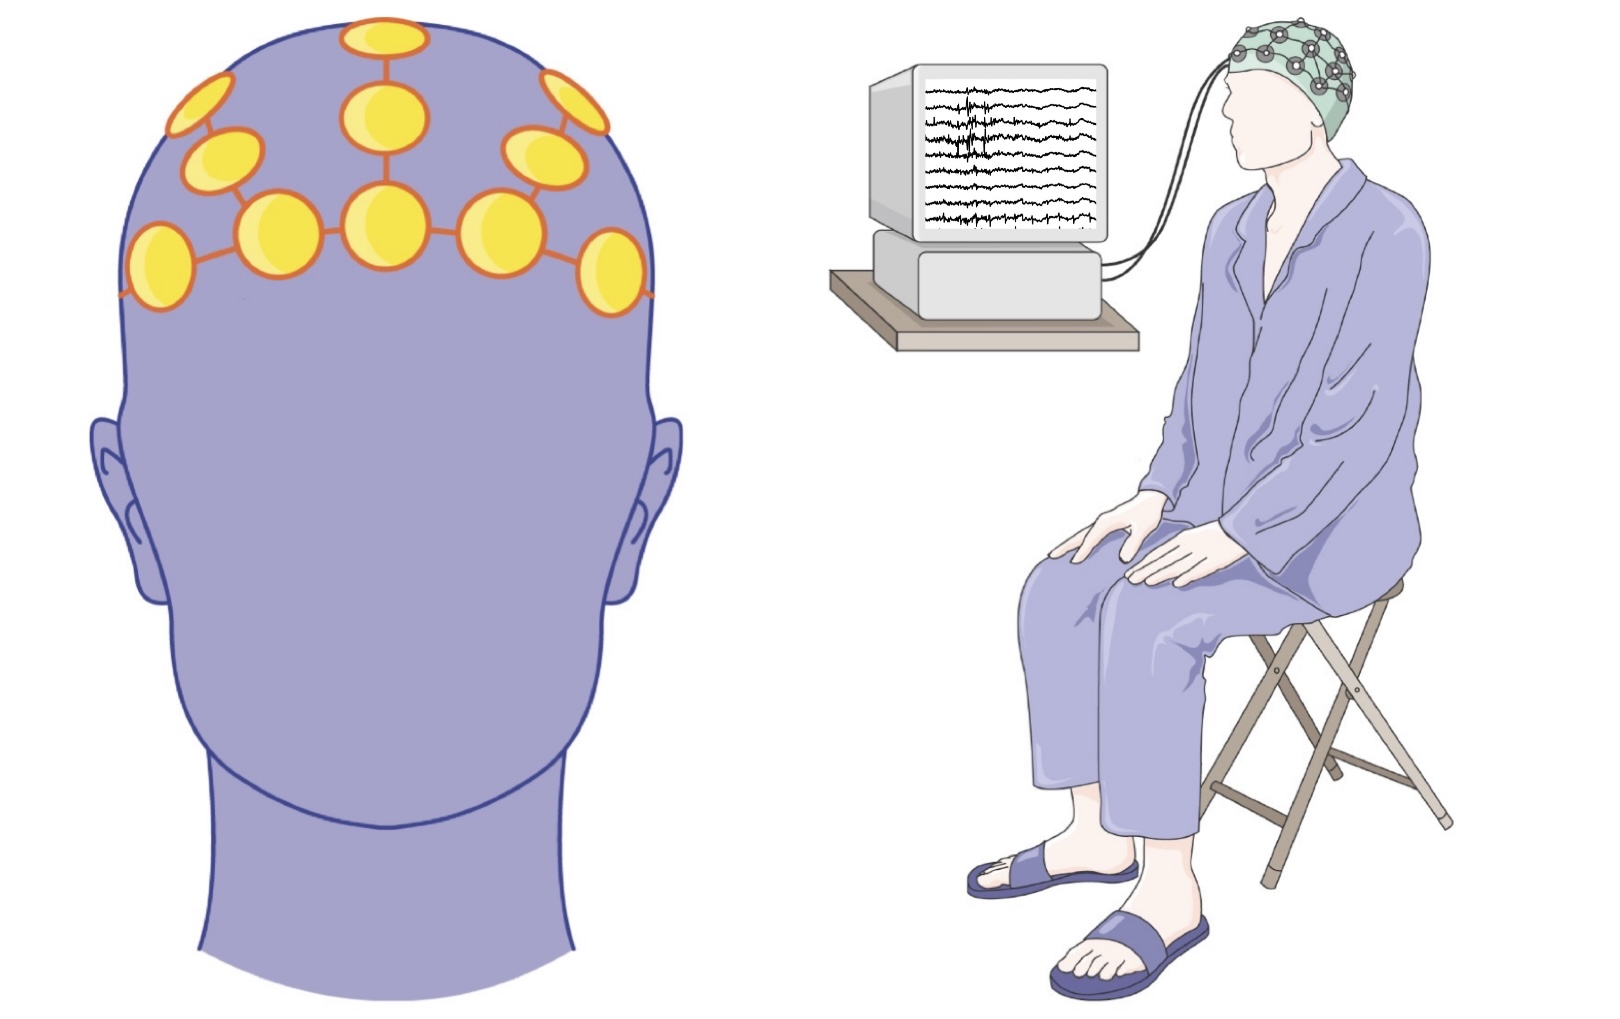
\includegraphics[width=0.6\linewidth]{figures/new_eeg_wiki.jpg}
    \caption{Illustration of the EEG method. The figures have been adapted from Wikimedia Commons with attribution to SMART-Servier Medical Art and are licensed under the Creative Commons Attribution-Share Alike 3.0 Unported license \cite{EEG_head} \cite{EEG_full_body}. The figures have been edited to remove some of the original details.}
    \label{fig:EEG}
\end{figure}

Electrical potentials generated by individual neurons are far too small to be picked up by the recording electrodes. Therefore EEG measurements primarily reflect the summation of synchronous activity from thousands of pyramidal neurons with similar spatial orientation. The activity originating from neurons with different geometric alignments cannot be picked up because their individual electrical signals tend to cancel each other out, resulting in undetectable waves at the scalp electrodes \cite{bromfield2006introduction}. The EEG is typically described in terms of rhythmic activity and transients, which are divided into frequency bands that can be extracted using spectral methods. Most of the cerebral signals observed in the scalp EEG fall within the range of 1–20 Hz.

Abnormal activity can broadly be classified into \emph{epileptiform} and \emph{non-epileptiform} activity. Epileptiform activity typically arises in EEG recordings of patients with epilepsy and includes spikes and sharp waves, that can be seen synchronously throughout the entire brain. In this context, spikes refer to hypersynchronized bursts from a sufficient number of neurons, arising from high-frequency bursts of action potentials \cite{bromfield2006introduction}.

Detecting and localizing abnormal electrical patterns in EEG represents an important research pursuit. One of the fundamental aspects in this field is the \emph{EEG inverse problem}, which is concerned with localizing brain activity of interest using EEG recordings. Further in this chapter, we will explore the concept of the EEG inverse problem and how to solve it. However, before delving into this concept, we will take a look at the subject of head models and the dipole approximation for the pupose of simulating EEG recordings, which in turn can be used in artificial neural networks for the purpose of solving the EEG inverse problem.

\section{Head Models}
To accurately simulate EEG data, head models that faithfully represent the conductivity distribution within the human head can be utilized. Head models serve as computational representations of the head's anatomical structure, commonly encompassing the brain, skull, cerebrospinal fluid, and scalp.

The intricate biophysical properties of the head significantly impact EEG signals. Detailed head models play an important role in simulating the propagation of electrical signals through various tissue compartments, thus enabling the recreation of realistic neuronal activity.
For instance, the cerebrospinal fluid within the human brain exhibits a conductivity of approximately 1.7 S/m, while the skull and scalp possess conductivities of about 0.01 S/m and 0.5 S/m, respectively \cite{naess2021biophysically}.
These conductivity variations underscore the necessity for comprehensive head models that can account for such differences, thereby elucidating the intricate path of electrical signal propagation. In addition to conductivity considerations, detailed head models often incorporate the influence of tissue arrangement on EEG signals, such as whether a neuronal population is located within a sulcus or a gyrus \cite{naess2021biophysically}.


\subsection{The Current Dipole Approximation}
In the context of head models, neural activity is often represented through the simulation of current dipoles. The concept of the \emph{current dipole approximation} is rooted in the observation that, as the distance from the neuron to the extracellular potential $V_e$ increases, the neural contribution becomes increasingly more dipole-like.

The key insight behind the current dipole approximation lies in the \emph{multipole expansion}, a technique that comes to our aid when the recording point is situated at a significant distance from the source distribution. While electrical charges within neural tissue can give rise to the formation of current multipoles, the multipole expansion theorem offers a method to express the extracellular potential $V_e$ in terms of various pole contributions. In the context of EEG signals, employing this theorem reveals that $V_e$ can be effectively approximated by a single dipole \cite{brainmodel2022}.

Neuronal multipoles depend on the spatial arrangement and symmetry of the charge distribution and result from the interplay of current sources and sinks \cite{wiki:multipoles}. The expression for the extracellular potential associated with different multipole orders may take complicated forms, and be hard to interpreted. However, when the distance $R$ from the center of the source to the recording point surpasses the extent of the source, the tequniqe of multipole expansion can be utilized \cite{jackson1999classical}. This expansion are often beneficial as usually only the first few terms are needed in order to provide an accurate approximation of the original funtion, as we will se now. Using the multipole expansion theorem, the representation of the extracellular potential $V_e(R)$ takes the form:

\begin{equation}
  V_e(R) = \frac{C_{\text{monopole}}}{R} + \frac{C_{\text{dipole}}}{R^2} + \frac{C_{\text{quadrupole}}}{R^3} + \frac{C_{\text{octopole}}}{R^4} + ... .
\label{eq:extracellular_potential}
\end{equation}

where the numerators represents the contributions to the extracellular potential. The terms denoted $C_\text{monopole}$, $C_\text{dipole}$ and $C_\text{quadrupole}$ represents contributions to the extracellulat potential $V_e$ and can in general be extremely complicated as they depend on the relationship between radial coordinates and symmetry of the current source and measurement electrode. We note that the contributions beyond the dipole term decay more rapidly with distance $R$. This means that in scenarios where we are considerably distant from the source distribution, the higher-order terms become negligible, leaving us primarily with the monopole and dipole contribution. However, as the net sum of currents over a neuronal membrane is invariably zero, the monopole contribution also vanishes. Consequently, we are left with an approximation of the extracellular potential, $V_e$, that relies solely on the dipole contribution:

\begin{equation}
V_e(\textbf{r}) \approx \frac{C_{\text{dipole}}}{R^2} = \frac{1}{4\pi\sigma}\frac{|\textbf{p}| \text{cos} \theta}{\lvert\textbf{r}-\textbf{r}_p\rvert^2}.
\label{eq:extracellular_potential_approximation}
\end{equation}

Here we have substituded for $C_\text{dipole}$ in terms of other properties, where $p$ is the current dipole moment within a medium of conductivity $\sigma$. The distance between the current dipole moment at $\textbf{r}_p$ and the electrode location $\textbf{r}$ is denoted as $R = |\textbf{R}| = |\textbf{r} - \textbf{r}_p|$. Additionally, $\theta$ signifies the angle between $\textbf{p}$ and $\textbf{R}$. This equation is recognized as the dipole approximation and stands as a reliable method for calculating the extracellular potential, particularly when the distance $R$ significantly surpasses the dipole length. This condition is inevitably met in EEG studies, as the dipole length cannot exceed the depth of the cortex, while EEG electrodes are typically positioned several centimeters away from the cortical surface on the scalp \cite{naess2021biophysically}.

In Figure \ref{fig:dipole_pattern}, we have provided a simulation of the extracellular potential generated by a neuron in response to a single synaptic input, where the spatial distribution of membrane current was explicitly taken into consideration. The Figure has been collected from work done by Torbjørn Ness and Gaute Einevoll. This simulation aligns with the dipole approximation, as it clearly visualizes the distribution of electric charge in the extracellular potential of the neuron's surroundings, revealing distinct dipole patterns when observed from a greater distance.

\begin{figure}
    \centering
    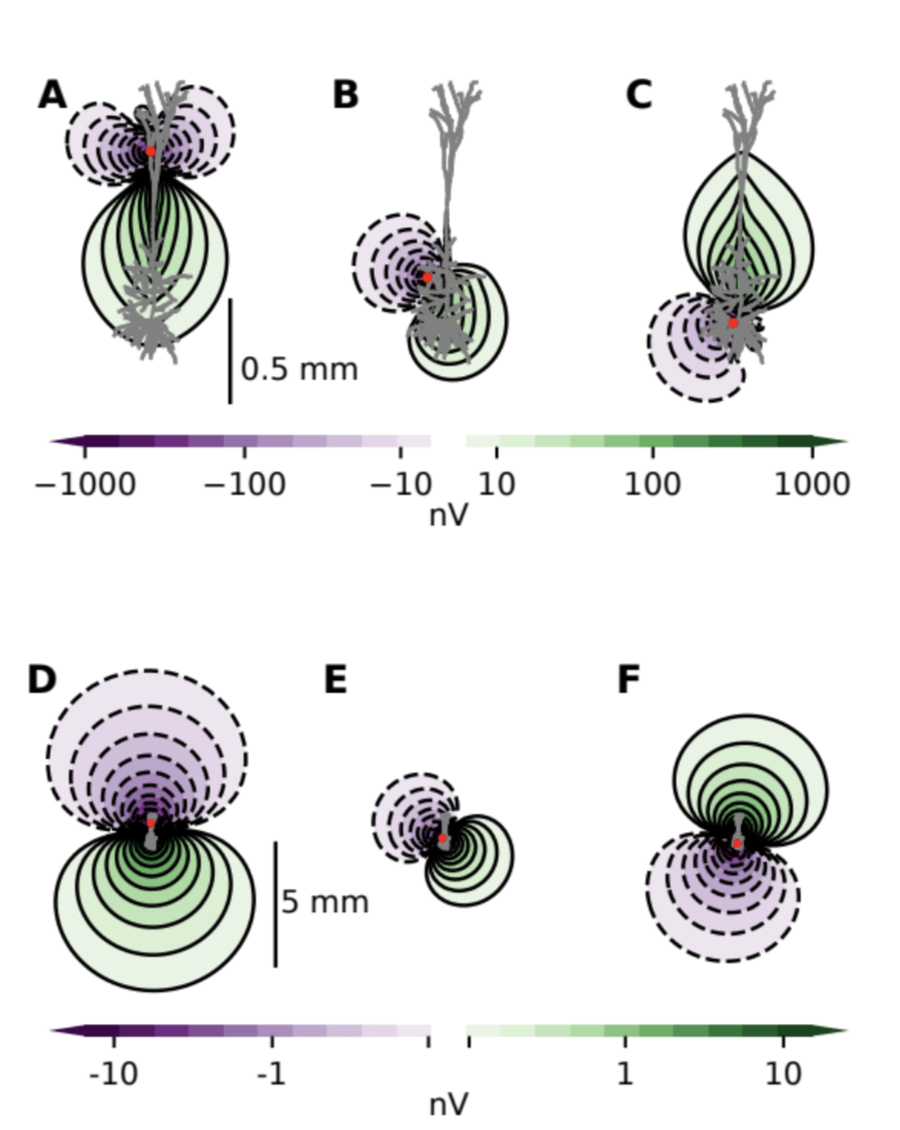
\includegraphics[width=\linewidth]{figures/dipole_pattern.png}
    \caption{Simulation of extracellulat potential showing distinct dipole pattern. The figure belongs to work carried out by Torbjørn Ness and Gaute Einevoll.}
    \label{fig:dipole_pattern}
\end{figure}



\subsection{The New York Head Model}
The New York Head Model (NYHM), developed by the Biomedical Engineering Department at the City University of New York \cite{huang2016new}, is a highly detailed computer model designed for simulating electrical brain activity, with a focus on EEG source localization. Grounded in high-resolution anatomical MRI data from 152 adult heads, this model enables the segmentation of six distinct tissue types within the head: scalp, skull, cerebrospinal fluid, gray matter, white matter, and air cavities. Its high level of detail and accuracy makes it an appropriate tool for simulating and understanding brain activity realistically. Providing a three-dimensional representation of the head and brain, along with precise information about tissue geometry and electrical properties, this head model will be employed in our work within the context of EEG simulation to generate the data used for dipole source localization.

To accurately calculate EEG signals recorded at various scalp locations, head models typically compute what is commonly referred to as a model-specific \emph{lead field matrix} \(L\). A lead field can be thought of as a geometric arrangement that links the sensitivity of EEG measurements from various scalp locations to potential neural current sources within the brain. The lead field matrix of the NYHM is computed for 231 electrode positions on the scalp and 74,382 possible dipole source locations within the cortex. Each location point includes the \(x\)-, \(y\)-, and \(z\)-coordinates, with the \(x\)-coordinate ranging from -72 to 72 mm, the \(y\)-coordinate spanning -106 to 73 mm, and the \(z\)-coordinate extending from -53 to 82 mm. Mathematically, the lead field matrix can be defined as:
\begin{equation}
  L_{ij} = \frac{E_j^{(i)}}{I}, \quad \text{for } j = x, y, z.
  \label{eq:LeadFieldMatrix}
\end{equation}
Here, \(I\) represents the injected current at the electrode locations, and \({E}^{(i)} = (E_x^{(i)}, E_y^{(i)}, E_z^{(i)})\) is the resulting electric field in the brain. The row index \(i\) spans from 1 to \(231 \times 74,382\).

The \emph{forward modeling} of the EEG signal \(\Phi\) can be described through a straightforward matrix multiplication:
\begin{equation}
  \Phi = L \mathbf{p},
  \label{eq:EEG_signal_matrix}
\end{equation}
where, the current dipole moment \(\mathbf{p} = (p_x, p_y, p_z)\) represents the dipole's magnitude in the \(x\), \(y\), and \(z\)-directions, respectively. In the context of the NYHM, a forward configuration of an EEG signal encompasses the 231 values measured at each of the scalp electrodes resulting from a current dipole \(\mathbf{p}\).

For more comprehensive details about the New York Head Model, we recommend referring to Huang, Parra, and Haufe (2016) \cite{huang2016new}.




\rednote{Usikker på om dette bør flyttes til neste kapittel?}
\subsection{The Effect of Dipole Orientation}
Figure \ref{fig:gyrus_and_sulcus_EEG} and \ref{fig:dipole_orientation} are borrowed from work done by Tornjørn Ness and Gaute Einevoll, and illustrate the impact of dipole orientation on EEG outcomes within the NYHM. Figure \ref{fig:gyrus_and_sulcus_EEG} represent the EEG signals obtained from two manually selected dipole locations. These dipoles are situated in a gyrus and a sulcus, respectively, and exhibit distinct EEG patterns. In general, the contribution of an individual current dipole to the EEG signal is maximized when the dipole is perpendicularly situated within a gyrus, as depicted in Figure \ref{fig:gyrus_and_sulcus_EEG}B. Contrastingly, when a dipole is placed in a sulcus with a perpendicular orientation, a significant EEG contribution may still be observed, however unlike the dipole in the gyrus, it exhibits a more dipolar pattern, as shown in Figure \ref{fig:gyrus_and_sulcus_EEG}C.


\begin{figure}[!htb]
    \centering
    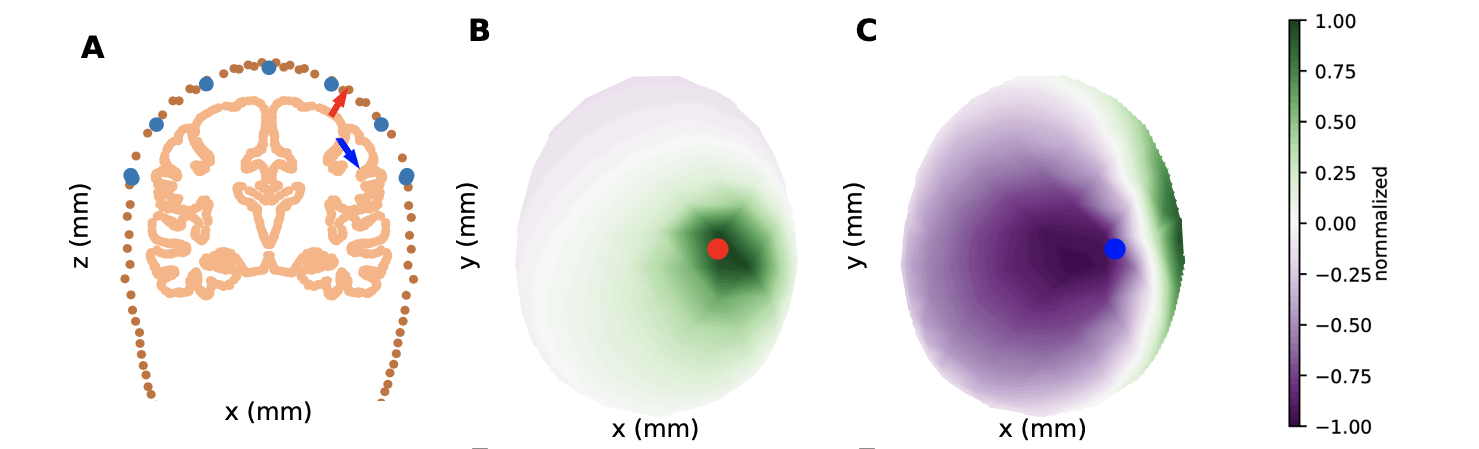
\includegraphics[width=\linewidth]{figures/gyrus_and_sulcus_EEG.png}
    \caption{A: Two selected dipole locations in the New York head model: one in a gyrus (red) and one in a sulcus (blue). The head model is viewed from the side (x, z-plane). Close to the chosen cross-section plane, EEG electrode locations are marked in light blue. Available dipole locations near the cortical cross-section form an outline of the cortical sheet and are marked in pink. The current dipole moment for all cases was 1 nAm. B: Interpolated color plot of EEG signal from the gyrus dipole, viewed from the top (x, y-plane). The plotted EEG signal is scaled, with a maximum value of 1.1 $\mu$V. C: Interpolated color plot of EEG signal from the sulcus dipole. The plotted EEG signal is scaled, with a maximum value of 0.7 $\mu$V. This Figure is borrowed from work done by Torbjørn Ness and Gaute Einevoll \cite{naess2021biophysically}.}
    \label{fig:gyrus_and_sulcus_EEG}
\end{figure}

Further, Figure \ref{fig:dipole_orientation} depicts the EEG signals from identical dipoles positioned in various folding patterns of the cortical surface. These patterns align with the previous observations, as they showcases that the orientation of the current dipole moment significantly influences the EEG outcome. Firstly, Figure \ref{fig:dipole_orientation}A and \ref{fig:dipole_orientation}C provide an expanded illustration of the aforementioned scenarios, incorporating additional dipole moments located in a gyrus and a sulcus, respectively. In Figure \ref{fig:dipole_orientation}B, where a collection of dipoles points randomly upwards and downwards, the EEG signal contribution appears to diminish significantly. Conversely, when the dipoles align in the depth direction of the cortex and are distributed across both gyrus and sulcus, we can expect an EEG contribution in between what we saw from Figure \ref{fig:dipole_orientation}A and \ref{fig:dipole_orientation}B, as depicted in Figure \ref{fig:dipole_orientation}D. Lastly, Figure \ref{fig:dipole_orientation}E demonstrates the minimal EEG contribution observed when the dipoles are divided between two opposing sulci.


\begin{figure}[!htb]
    \centering
    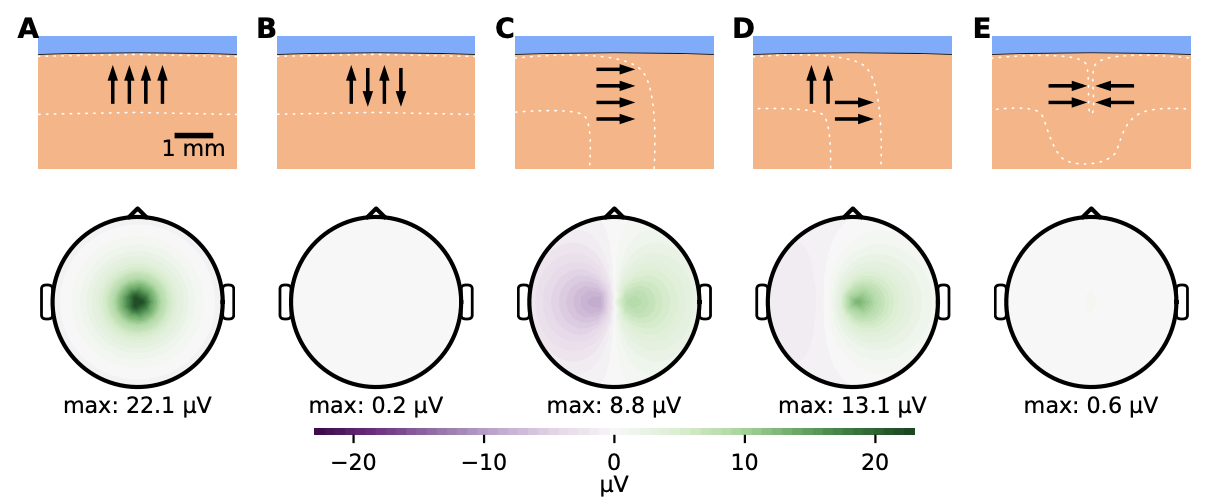
\includegraphics[width=\linewidth]{figures/dipole_orientation.png}
    \caption{Different folding patterns of the cortical surface are represented by white dashed lines. EEG signals are calculated from four identical current dipoles with varying orientations. A: Dipoles aligned in the same direction within a gyrus. B: Dipoles pointing in opposite directions within a gyrus. C: Dipoles aligned in the same direction within a sulcus. D: Dipoles distributed between a gyrus and a sulcus, pointing towards the cortical surface. E: Dipoles divided between opposing sulci, pointing towards the cortical surface.
    Each panel features a dipole moment magnitude of 10 nAm, and the dipoles are positioned at the centers of the arrows in the top row. This Figure is borrowed from work done by Torbjørn Ness and Gaute Einevoll \cite{naess2021biophysically}.}
    \label{fig:dipole_orientation}
\end{figure}



\section{The Inverse Problem and Source Localization}
In the field of neuroscience, the inverse problem involves locating the underlying neural activity responsible for a set of measured EEG data. In contrast to the \emph{forward problem}, where known parameters are used to predict the resulting EEG potential, the inverse problem lacks a unique solution. This implies that different configurations of neural sources can produce the same EEG activity distribution on the scalp \cite{hecker2021convdip}.

The EEG inverse problem can be mathematically formulated as follows:
\begin{equation}
\mathbf{p} = {L}^{-1} \cdot {\Phi},
\label{eq:inverse_problem}
\end{equation}
Here, \(\mathbf{L}^{-1}\) denotes the inverse of the lead field matrix.

Machine learning techniques such as artificial neural networks can be used to estimate probable source locations by learning patterns from large datasets of EEG recordings and corresponding source locations, which can be simulated through forward modeling using head models. Neural network approaches for solving the inverse problem have been identified as yielding faster inverse solutions than classical methods \cite{sclabassi2001eeg}.

In the next chapter, we will take a practical step by simulating EEG data using the New York Head Model. This simulated data will lay the foundation for the development of neural networks in the following chapters, with the purpose of addressing the EEG inverse problem.

\end{document}

